% freak cheat sheet: one landscape A4 card.  Build: make cheatsheet
% Every number here comes from lib/launchkey_ctl.h and lib/freak_dsp.h.
\documentclass{article}
\usepackage[a4paper,landscape,margin=6mm]{geometry}
\usepackage[T1]{fontenc}
\usepackage{lmodern}
\usepackage[default]{sourcesanspro}
\usepackage{amssymb}
\usepackage{tikz}
\usepackage[most]{tcolorbox}
\usepackage{array}
\usepackage{tabularx}
\pagestyle{empty}
\setlength{\parindent}{0pt}

\definecolor{ink}{RGB}{30,30,30}
\definecolor{snd}{RGB}{20,20,20}       % sound-page knob labels
\definecolor{fxc}{RGB}{30,90,170}      % FX-page knob labels
\definecolor{ampc}{RGB}{67,160,71}     % amp envelope
\definecolor{modc}{RGB}{230,140,20}    % mod envelope
\definecolor{lfoc}{RGB}{150,60,170}    % LFO
\definecolor{fltc}{RGB}{215,60,50}     % filter
\definecolor{freec}{RGB}{170,170,170}  % unassigned
\definecolor{padc}{RGB}{120,170,230}

\newcommand{\FX}[1]{\textcolor{fxc}{#1}}
\newcommand{\cc}[1]{\textcolor{black!45}{\fontsize{4.6}{5}\selectfont #1}}

% knob: x, SOUND label, FX label
\newcommand{\knob}[3]{%
  \draw[fill=black!8, draw=black!60, line width=0.4pt] (#1,62) circle (3.6);
  \draw[black!60, line width=0.5pt] (#1,62) -- ++(110:3.1);
  \node[font=\fontsize{5.6}{6.2}\selectfont\bfseries, text=snd, align=center] at (#1,69.4) {#2};
  \node[font=\fontsize{5.6}{6.2}\selectfont, text=fxc, align=center] at (#1,54.4) {#3};}
% pad: col (0..7), row (1 top, 0 bottom), label
\newcommand{\pad}[3]{%
  \draw[rounded corners=0.8mm, fill=padc!35!white, draw=padc!80!black, line width=0.4pt]
    (36+#1*13.2, 22+#2*13.2) rectangle ++(12,12);
  \node[font=\fontsize{5.4}{6}\selectfont, text=ink, align=center, text width=11mm]
    at (36+#1*13.2+6, 22+#2*13.2+6) {#3};}
% fader: x, top label, colour
\newcommand{\fader}[3]{%
  \draw[fill=black!12, draw=black!50] (#1-0.7,26) rectangle (#1+0.7,52);
  \draw[fill=#3!60!white, draw=#3!70!black, rounded corners=0.4mm] (#1-2.6,36) rectangle (#1+2.6,40);
  \node[font=\fontsize{5.6}{6.2}\selectfont\bfseries, text=#3!70!black, align=center] at (#1,56) {#2};}
% small button: x, y, label, colour, width
\newcommand{\btn}[5]{%
  \draw[rounded corners=0.6mm, fill=#4!25!white, draw=#4!70!black, line width=0.4pt]
    (#1-#5/2,#2-2.6) rectangle (#1+#5/2,#2+2.6);
  \node[font=\fontsize{4.9}{5.4}\selectfont, text=ink, align=center] at (#1,#2) {#3};}

\tcbset{card/.style={enhanced, colback=white, colframe=black!70, boxrule=0.5pt, arc=1.5mm,
    left=1.6mm, right=1.6mm, top=1.1mm, bottom=1.1mm, toptitle=0.6mm, bottomtitle=0.6mm,
    fonttitle=\bfseries\fontsize{8.6}{10}\selectfont, coltitle=white, colbacktitle=black!75,
    fontupper=\fontsize{7.1}{8.5}\selectfont, before skip=0mm, after skip=1.8mm}}
\newtcolorbox{card}[1]{card, title={#1}}
\newcolumntype{L}{>{\raggedright\arraybackslash}X}

\begin{document}

{\fontsize{16}{18}\selectfont\bfseries freak}\hspace{3mm}%
{\fontsize{9.5}{11}\selectfont Axoloti Core + Launchkey 49 MK3 (standalone mode) \textperiodcentered{}
3-voice Braids synth \textperiodcentered{} patch \texttt{patches/freak/freak\_v1.axp}}\hfill
{\fontsize{7}{8}\selectfont\color{black!55} v1.1 \textperiodcentered{} 2026-11-04 \textperiodcentered{} page 1 of 2 \textperiodcentered{} github.com/ndlopes-github/axoloti-playground}

\vspace{1.5mm}
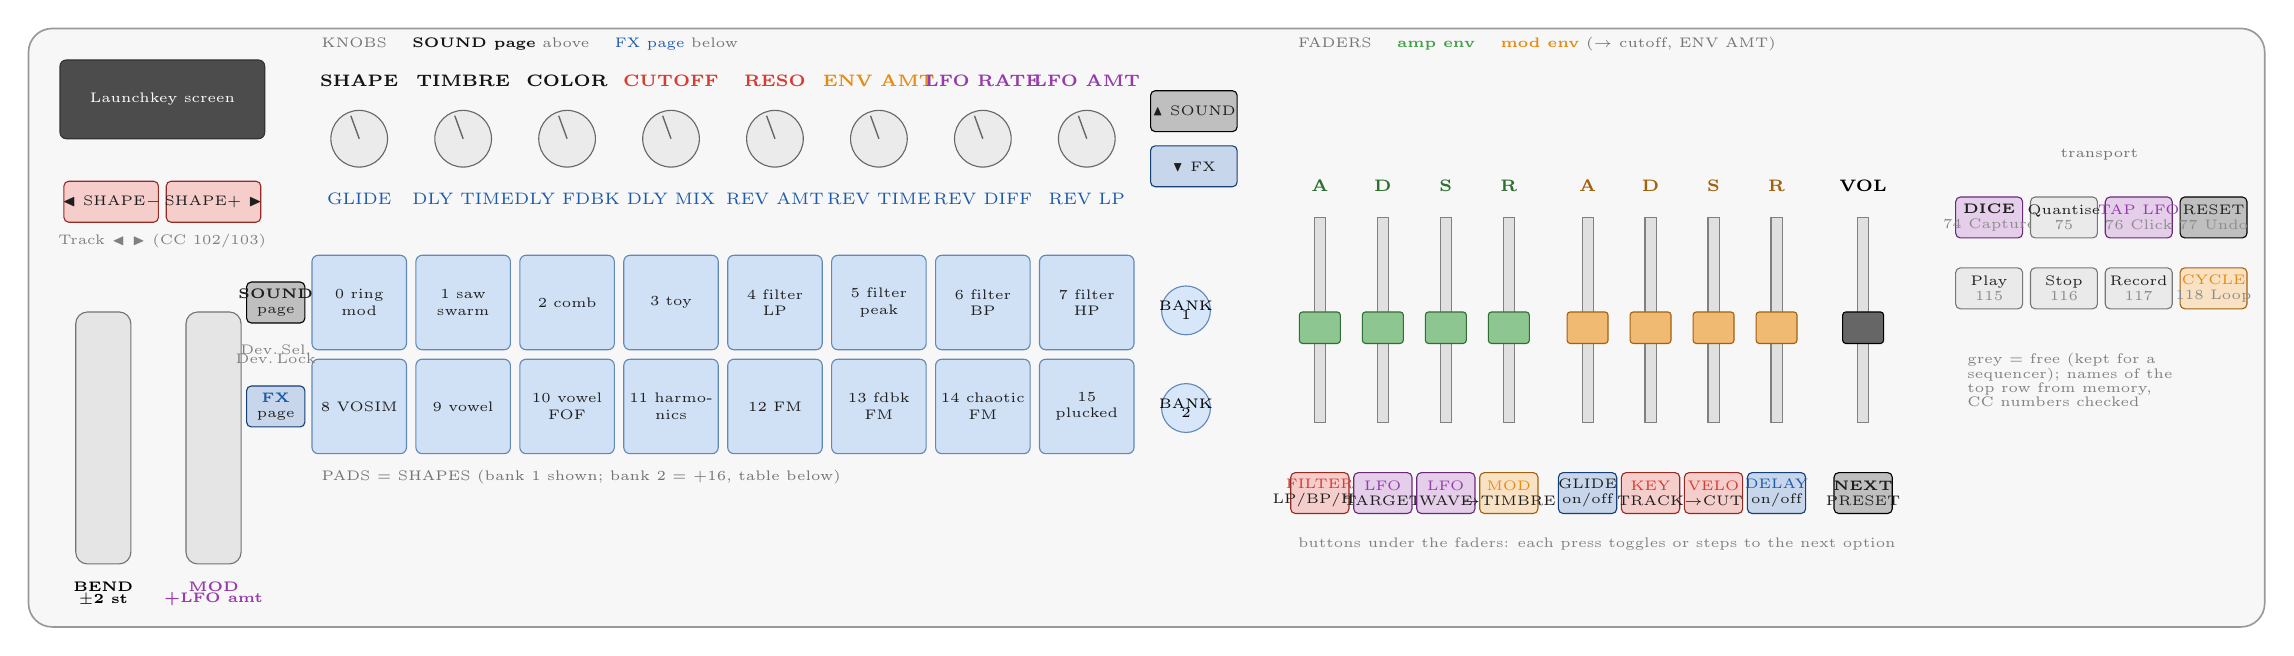
\begin{tikzpicture}[x=1mm,y=1mm]
  \draw[rounded corners=3mm, fill=black!3, draw=black!40, line width=0.6pt] (0,0) rectangle (284,76);

  % ---- left: screen, track buttons, wheels
  \draw[fill=black!70, draw=black!80, rounded corners=0.8mm] (4,62) rectangle (30,72);
  \node[font=\fontsize{5}{6}\selectfont, text=white] at (17,67) {Launchkey screen};
  \btn{10.5}{54}{\(\blacktriangleleft\) SHAPE\(-\)}{fltc}{12}
  \btn{23.5}{54}{SHAPE+ \(\blacktriangleright\)}{fltc}{12}
  \node[font=\fontsize{4.6}{5}\selectfont, text=black!50] at (17,49) {Track \(\blacktriangleleft\) \(\blacktriangleright\) (CC 102/103)};
  \draw[rounded corners=1.5mm, fill=black!10, draw=black!55] (6,8) rectangle (13,40);
  \draw[rounded corners=1.5mm, fill=black!10, draw=black!55] (20,8) rectangle (27,40);
  \node[font=\fontsize{5.4}{6}\selectfont\bfseries, align=center] at (9.5,4.2) {BEND\\[-0.6mm]\(\pm\)2 st};
  \node[font=\fontsize{5.4}{6}\selectfont\bfseries, align=center, text=lfoc] at (23.5,4.2) {MOD\\[-0.6mm]+LFO amt};

  % ---- knobs: SOUND page (black, top) / FX page (blue, below)
  \node[font=\fontsize{5}{6}\selectfont, text=black!55, anchor=west] at (36,74) {KNOBS \quad
     \textbf{\textcolor{snd}{SOUND page}} above \quad \textcolor{fxc}{FX page} below};
  \knob{42}{SHAPE}{\FX{GLIDE}}
  \knob{55.2}{TIMBRE}{\FX{DLY TIME}}
  \knob{68.4}{COLOR}{\FX{DLY FDBK}}
  \knob{81.6}{\textcolor{fltc}{CUTOFF}}{\FX{DLY MIX}}
  \knob{94.8}{\textcolor{fltc}{RESO}}{\FX{REV AMT}}
  \knob{108}{\textcolor{modc}{ENV AMT}}{\FX{REV TIME}}
  \knob{121.2}{\textcolor{lfoc}{LFO RATE}}{\FX{REV DIFF}}
  \knob{134.4}{\textcolor{lfoc}{LFO AMT}}{\FX{REV LP}}
  \btn{148}{65.5}{\(\blacktriangle\) SOUND}{black}{11}
  \btn{148}{58.5}{\(\blacktriangledown\) FX}{fxc}{11}

  % ---- pads (bank 1 shown) + side buttons
  \pad{0}{1}{0 ring\\mod}  \pad{1}{1}{1 saw\\swarm} \pad{2}{1}{2 comb}    \pad{3}{1}{3 toy}
  \pad{4}{1}{4 filter\\LP} \pad{5}{1}{5 filter\\peak} \pad{6}{1}{6 filter\\BP} \pad{7}{1}{7 filter\\HP}
  \pad{0}{0}{8 VOSIM}      \pad{1}{0}{9 vowel}    \pad{2}{0}{10 vowel\\FOF} \pad{3}{0}{11 harmo-\\nics}
  \pad{4}{0}{12 FM}        \pad{5}{0}{13 fdbk\\FM}  \pad{6}{0}{14 chaotic\\FM} \pad{7}{0}{15 plucked}
  \node[font=\fontsize{5}{6}\selectfont, text=black!55, anchor=west] at (36,19) {PADS = SHAPES (bank 1 shown; bank 2 = +16, table below)};
  % Device Select / Device Lock (CC 106/107): the knob pages
  \btn{31.4}{41.2}{\textbf{SOUND}\\page}{black}{7.4}
  \btn{31.4}{28}{\textbf{\FX{FX}}\\page}{fxc}{7.4}
  \node[font=\fontsize{4.2}{4.6}\selectfont, text=black!50, align=center] at (31.4,34.6) {Dev.\,Sel.\\[-0.5mm]Dev.\,Lock};
  \draw[fill=padc!30!white, draw=padc!80!black] (147,40.2) circle (3.1);
  \draw[fill=padc!30!white, draw=padc!80!black] (147,27.8) circle (3.1);
  \node[font=\fontsize{4.9}{5.4}\selectfont, align=center] at (147,40.2) {BANK\\[-0.8mm]1};
  \node[font=\fontsize{4.9}{5.4}\selectfont, align=center] at (147,27.8) {BANK\\[-0.8mm]2};

  % ---- faders
  \node[font=\fontsize{5}{6}\selectfont, text=black!55, anchor=west] at (160,74) {FADERS \quad
     \textcolor{ampc}{\textbf{amp env}} \quad \textcolor{modc}{\textbf{mod env}} (\(\to\) cutoff, ENV AMT)};
  \fader{164}{A}{ampc} \fader{172}{D}{ampc} \fader{180}{S}{ampc} \fader{188}{R}{ampc}
  \fader{198}{A}{modc} \fader{206}{D}{modc} \fader{214}{S}{modc} \fader{222}{R}{modc}
  \fader{233}{VOL}{black}
  % fader buttons (CC 11-19): press = toggle / next
  \btn{164}{17}{\textcolor{fltc}{FILTER}\\LP/BP/HP}{fltc}{7.4}
  \btn{172}{17}{\textcolor{lfoc}{LFO}\\TARGET}{lfoc}{7.4}
  \btn{180}{17}{\textcolor{lfoc}{LFO}\\WAVE}{lfoc}{7.4}
  \btn{188}{17}{\textcolor{modc}{MOD}\\\(\to\)TIMBRE}{modc}{7.4}
  \btn{198}{17}{GLIDE\\on/off}{fxc}{7.4}
  \btn{206}{17}{\textcolor{fltc}{KEY}\\TRACK}{fltc}{7.4}
  \btn{214}{17}{\textcolor{fltc}{VELO}\\\(\to\)CUT}{fltc}{7.4}
  \btn{222}{17}{\FX{DELAY}\\on/off}{fxc}{7.4}
  \btn{233}{17}{\textbf{NEXT}\\PRESET}{black}{7.4}
  \node[font=\fontsize{4.6}{5}\selectfont, text=black!50, anchor=west] at (160,10.5) {buttons under the faders: each press toggles or steps to the next option};

  % ---- transport (ch 16)
  \node[font=\fontsize{5}{6}\selectfont, text=black!55] at (263,60) {transport};
  \btn{249}{52}{\textbf{DICE}\\\cc{74 Capture}}{lfoc}{8.5}
  \btn{258.5}{52}{Quantise\\\cc{75}}{freec}{8.5}
  \btn{268}{52}{\textcolor{lfoc}{TAP LFO}\\\cc{76 Click}}{lfoc}{8.5}
  \btn{277.5}{52}{RESET\\\cc{77 Undo}}{black}{8.5}
  \btn{249}{43}{Play\\\cc{115}}{freec}{8.5}
  \btn{258.5}{43}{Stop\\\cc{116}}{freec}{8.5}
  \btn{268}{43}{Record\\\cc{117}}{freec}{8.5}
  \btn{277.5}{43}{\textcolor{modc}{CYCLE}\\\cc{118 Loop}}{modc}{8.5}
  \node[font=\fontsize{4.6}{5.2}\selectfont, text=black!50, align=left, anchor=north west] at (245,36)
     {grey = free (kept for a\\sequencer); names of the\\top row from memory,\\CC numbers checked};
\end{tikzpicture}

\vspace{1.2mm}
\begin{minipage}[t]{70mm}\vspace{0pt}
\begin{card}{Knobs: two pages, scaled pickup}
\begin{tabularx}{\linewidth}{@{}l L@{}}
\textbf{SHAPE} & 34 Braids shapes in turn (3--4 steps each) \\
\textbf{TIMBRE / COLOR} & the two Braids parameters (meaning depends on the shape) \\
\textbf{\textcolor{fltc}{CUTOFF}} & 20 Hz \(\cdot 2^{10k}\): 20 Hz -- 20 kHz \\
\textbf{\textcolor{fltc}{RESO}} & Q = 0.5 -- 20 (exponential) \\
\textbf{\textcolor{modc}{ENV AMT}} & mod env \(\to\) cutoff, \(\pm\)5 octaves, 0 at centre \\
\textbf{\textcolor{lfoc}{LFO RATE}} & 0.05 -- 20 Hz (or tap tempo) \\
\textbf{\textcolor{lfoc}{LFO AMT}} & 0 -- 1, plus the mod wheel \\[0.6mm]
\FX{GLIDE} & 0 -- 1 s (quadratic), with GLIDE on \\
\FX{DLY TIME / FDBK / MIX} & 10 ms -- 1.5 s; 0 -- 0.95; 0 -- 1 \\
\FX{REV AMT/TIME/DIFF/LP} & Elements reverb, 0 -- 1 each \\
\end{tabularx}
\vspace{0.6mm}
\textbf{Page: Device Select = SOUND, Device Lock = FX} (the two buttons left of the pads;
\(\blacktriangle\)/\(\blacktriangledown\) by the knobs do the same). A press always lands on a known page.
After a page change or RESET, a knob that is not where its value is still works: the value moves
\emph{proportionally} the way you turn and meets the knob at an end of travel at the latest. No jumps, no dead knobs.
FX knobs 1--4 are silent until GLIDE or DELAY is on.
\end{card}
\end{minipage}\hfill
\begin{minipage}[t]{68mm}\vspace{0pt}
\begin{card}{Envelopes and filter}
Faders 1--4 \textcolor{ampc}{\textbf{amp}}, 5--8 \textcolor{modc}{\textbf{mod}}: A, D, R =
1 ms \(\cdot 10^{4k}\) (1 ms -- 10 s, a decade per quarter of the travel); S = level 0 -- 1.
Exponential segments; attack aims at 1.2: a concave rise, fast at first (analog style).\\[0.5mm]
\textcolor{modc}{\textbf{Mod env}} \(\to\) cutoff (ENV AMT), and \(\to\) timbre (\(\pm\)0.5) with
MOD\(\to\)TIMBRE. \textcolor{modc}{\textbf{CYCLE}} (Loop): it loops attack/decay while a key is held.\\[0.5mm]
\textcolor{fltc}{\textbf{Filter}}: 12 dB/oct state-variable (LP/BP/HP, BP normalised).
KEY TRACK (on at power-on): cutoff follows the keys, 1 oct/oct around note 60 (middle C).
VELO\(\to\)CUT: up to +2 octaves for a hard hit.
\end{card}
\begin{card}{LFO (one, shared by the voices)}
TARGET: \textbf{timbre} \(\to\) color \(\to\) cutoff (\(\pm\)3 oct) \(\to\) pitch (\(\pm\)2 st).\quad
WAVE: \textbf{sine} \(\to\) triangle \(\to\) saw \(\to\) square \(\to\) S\&H.\quad
TAP LFO: two taps 0.1--4 s apart set the period; LFO RATE takes over again when turned.
\end{card}
\end{minipage}\hfill
\begin{minipage}[t]{66mm}\vspace{0pt}
\begin{card}{Pads: shapes, two banks}
\fontsize{6.4}{7.4}\selectfont
\begin{tabularx}{\linewidth}{@{}L L@{}}
\textbf{Bank 1} (0--15) & \textbf{Bank 2} (16--31) \\
0 ring mod \quad 1 saw swarm & 16 bowed \quad 17 blown \\
2 comb \quad 3 toy & 18 fluted \quad 19 bell \\
4--7 filter LP/peak/BP/HP & 20 drum \quad 21 kick \\
8 VOSIM \quad 9 vowel & 22 cymbal \quad 23 snare \\
10 vowel FOF \quad 11 harmonics & 24 wavetables \quad 25 wave map \\
12 FM \quad 13 feedback FM & 26 wave line \quad 27 paraphonic \\
14 chaotic FM \quad 15 plucked & 28 filtered noise \quad 29 twin peaks \\
 & 30 clocked noise \quad 31 granular \\
\end{tabularx}
Top row = first 8, bottom row = next 8. 32 particle noise and 33 digital modulation:
\(\blacktriangleright\) from 31, or the SHAPE knob. Strike-type shapes (plucked, bell, drums)
are struck on each key press.
\end{card}
\begin{card}{Notes}
3 voices (a 4th note takes the oldest voice). \textbf{NEXT PRESET} (fader button 9) steps through
8 presets (page 2); \textbf{RESET} (Undo) is preset 0, the power-on sound; \textbf{DICE} (Capture MIDI)
rolls a random SOUND page and keeps envelope, FX and volume. Controls left behind by a preset or a roll
pick up smoothly. Toggle states are \textbf{not shown} yet (no LEDs in standalone mode).
\end{card}
\end{minipage}\hfill
\begin{minipage}[t]{63mm}\vspace{0pt}
\begin{card}{The Launchkey's own features}
They make notes, so they play freak as well (set them on the Launchkey, see its user guide):\\[0.4mm]
\textbf{Arp}: up, down, up/down, as played, random, chord, mutate; 1/4 -- 1/32T; 1--4 oct;
latch, gate, swing, rhythm.\\
\textbf{Scale}: minor, major, \textbf{Dorian}, \textbf{Mixolydian}, Phrygian, harmonic minor,
minor/major pentatonic.\\
\textbf{Fixed chord}, octave \(\pm\), transpose.\\[0.4mm]
{\color{black!55} Not yet tested with freak.}
\end{card}
\begin{card}{Signal path and load}
3 \(\times\) (Braids \(\to\) SVF \(\to\) amp env \(\times\) velocity) \(\to\) delay \(\to\)
Elements reverb \(\to\) VOL. Velocity: soft notes keep \(\frac14\) of the level.
DSP 57\,\%, patch RAM 40 of 44 KB (Axoloti Core, Ksoloti 1.1.0).
\end{card}
\end{minipage}

%======================================================================
\newpage
{\fontsize{16}{18}\selectfont\bfseries freak}\hspace{3mm}%
{\fontsize{9.5}{11}\selectfont shapes, dial values, presets, troubleshooting}\hfill
{\fontsize{7}{8}\selectfont\color{black!55} v1.1 \textperiodcentered{} page 2 of 2}

\vspace{1.5mm}
\newcommand{\sh}[5]{#1 & \textcolor{black!55}{#2} & \textbf{#3} & #4 & #5 \\}
\begin{minipage}[t]{166mm}\vspace{0pt}
\begin{card}{The 34 shapes: what TIMBRE (knob 2) and COLOR (knob 3) do \quad\textmd{\fontsize{6.5}{7}\selectfont (after the Braids manual)}}
\fontsize{6.9}{8.3}\selectfont
\setlength{\tabcolsep}{2.4pt}
\begin{tabular}[t]{@{}r l l l l@{}}
\# & pad & shape & TIMBRE & COLOR \\ \hline
\sh{0}{1·T1}{ring mod}{tuning of sines 2, 3}{tuning of sines 2, 3}
\sh{1}{1·T2}{saw swarm}{detune (7 saws)}{high-pass}
\sh{2}{1·T3}{comb}{comb pitch}{feedback \(-\)\,/\,0\,/\,+ (L\,/\,noon\,/\,R)}
\sh{3}{1·T4}{toy}{clock rate}{glitches}
\sh{4}{1·T5}{filter LP}{cutoff}{wave: saw\(\to\)square\(\to\)tri}
\sh{5}{1·T6}{filter peak}{cutoff}{wave: saw\(\to\)square\(\to\)tri}
\sh{6}{1·T7}{filter BP}{cutoff}{wave: saw\(\to\)square\(\to\)tri}
\sh{7}{1·T8}{filter HP}{cutoff}{wave: saw\(\to\)square\(\to\)tri}
\sh{8}{1·B1}{VOSIM}{formant 1}{formant 2}
\sh{9}{1·B2}{vowel}{vowel a e i o u}{formant shift}
\sh{10}{1·B3}{vowel FOF}{vowel a e i o u}{formant shift}
\sh{11}{1·B4}{harmonics}{centre of the 12 harmonics}{their spread}
\sh{12}{1·B5}{FM}{mod amount}{ratio}
\sh{13}{1·B6}{feedback FM}{mod amount (harsher)}{ratio}
\sh{14}{1·B7}{chaotic FM}{mod amount (unstable)}{ratio}
\sh{15}{1·B8}{plucked}{damping}{pluck position}
\sh{16}{2·T1}{bowed}{friction}{bow position}
\end{tabular}\hfill
\begin{tabular}[t]{@{}r l l l l@{}}
\# & pad & shape & TIMBRE & COLOR \\ \hline
\sh{17}{2·T2}{blown}{air pressure}{geometry}
\sh{18}{2·T3}{fluted}{air pressure}{geometry}
\sh{19}{2·T4}{bell}{damping}{inharmonicity}
\sh{20}{2·T5}{drum}{damping}{brightness}
\sh{21}{2·T6}{kick}{decay}{tone}
\sh{22}{2·T7}{cymbal}{band-pass cutoff}{drone \(\leftrightarrow\) noise}
\sh{23}{2·T8}{snare}{tone}{snappy (noise)}
\sh{24}{2·B1}{wavetables}{sweep the table}{table, 1 of 20}
\sh{25}{2·B2}{wave map}{X in a 16\(\times\)16 map}{Y}
\sh{26}{2·B3}{wave line}{position}{smoothing (left: stepped)}
\sh{27}{2·B4}{paraphonic}{wave}{\textbf{chord} (left: unison)}
\sh{28}{2·B5}{filtered noise}{resonance}{LP \(\leftrightarrow\) HP; keys = cutoff}
\sh{29}{2·B6}{twin peaks}{resonance Q}{peak spacing}
\sh{30}{2·B7}{clocked noise}{periodicity}{quantise 2--32 steps}
\sh{31}{2·B8}{granular}{grain density}{pitch randomness}
\sh{32}{\(\blacktriangleright\)}{particles}{density}{pitch randomness}
\sh{33}{\(\blacktriangleright\)}{digital mod}{bit rate}{data byte}
\end{tabular}\\[0.6mm]
pad = bank\(\cdot\)row+column: 1\(\cdot\)T1 is bank 1, top row, first pad (BANK 1/2 = the round buttons right of the pads).
Plucked, bowed, bell, drum, kick, cymbal and snare are struck on each new key: S and R shape the tail only.
Time constants inside Braids that do not follow pitch (grain rates, built-in decays) run at half the original speed.
\end{card}

\begin{card}{Presets: NEXT PRESET (fader button 9) steps 0\(\to\)7\(\to\)0, RESET (Undo) = 0 \quad\textmd{\fontsize{6.5}{7}\selectfont (chosen from the parameter meanings, not yet tuned by ear)}}
\fontsize{7.2}{8.7}\selectfont
\begin{tabularx}{\linewidth}{@{}>{\bfseries}l L@{}}
0 init & saw swarm, LP, key tracking; delay off. The power-on sound. \\
1 vowel pad & vowel FOF; attack 0.5 s, release 1 s; LFO\(\to\)timbre, sine, 0.2 Hz, 1/3 deep; cutoff 3.6 kHz;
delay 0.12 s (fdbk 0.3, mix 1/4), reverb 1/2. Nu-jazz pads. \\
2 FM bass & FM, light modulation; plucky amp (decay 0.1 s, no sustain); low-pass at 200 Hz (note 60) opened
+2.5 oct by the mod env; velocity\(\to\)cutoff; 60 ms glide. Play low: broken-beat bass. \\
3 glass mallets & bell, long ring, nearly harmonic; high-pass at 113 Hz; release 1 s; big reverb. \\
4 chord stabs & paraphonic: each key plays a chord (COLOR picks it); short stabs; delay 0.43 s, fdbk 0.48. \\
5 granular weather & granular, random grain pitch; band-pass; LFO S\&H\(\to\)color; CYCLE on: swelling, shifting texture. \\
6 pitched rain & particles, wide pitch spread; long delay feedback (0.71), big reverb. \\
7 chaotic drone & chaotic FM; attack 0.7 s, release 1.4 s; band-pass with a slow triangle LFO (0.13 Hz) on cutoff;
CYCLE on; long delay and reverb. Hold a chord. \\
\end{tabularx}\\[0.3mm]
A preset changes both knob pages, faders 1--8, the shape and the toggles; the volume stays. \textbf{DICE}
(Capture MIDI) rolls a random SOUND page instead. Controls that a preset or roll left behind pick up smoothly.
\end{card}
\end{minipage}\hfill
\begin{minipage}[t]{112mm}\vspace{0pt}
\begin{card}{Where the values fall (knob or fader turned \dots)}
\fontsize{7.5}{9.2}\selectfont
\setlength{\tabcolsep}{3pt}
\begin{tabular}{@{}l r r r r@{}}
 & 1/4 & 1/2 & 3/4 & full \\ \hline
\textcolor{ampc}{\textbf{A}}, \textcolor{ampc}{\textbf{D}}, \textcolor{ampc}{\textbf{R}} (both envelopes) & 10 ms & 100 ms & 1 s & 10 s \\
\textcolor{fltc}{\textbf{CUTOFF}} (at note 60) & 113 Hz & 640 Hz & 3.6 kHz & 20 kHz \\
\textcolor{fltc}{\textbf{RESO}} (Q) & 1.3 & 3.2 & 8 & 20 \\
\textcolor{modc}{\textbf{ENV AMT}} & \(-\)2.5 oct & 0 & +2.5 oct & +5 oct \\
\textcolor{lfoc}{\textbf{LFO RATE}} & 0.22 Hz & 1 Hz & 4.5 Hz & 20 Hz \\
\FX{GLIDE} & 0.06 s & 0.25 s & 0.56 s & 1 s \\
\FX{DLY TIME} & 35 ms & 0.12 s & 0.43 s & 1.5 s \\
\FX{DLY FDBK} & 0.24 & 0.48 & 0.71 & 0.95 \\
\textbf{VOL} (gain) & 0.06 & 0.25 & 0.56 & 1 \\
\end{tabular}\\[0.5mm]
Times are exponential: each quarter of the travel is a factor of 10. S, TIMBRE, COLOR and the mixes are linear, 0--1.
\end{card}

\begin{card}{Something seems wrong?}
\fontsize{7.5}{9.2}\selectfont
\textbf{No sound}: VOL (fader 9) up? CUTOFF (knob 4) not at the bottom in LP, nor at the top in HP?
A struck shape (pluck, bell, drums) only sounds on a new key. Is the patch running (Live / startup)?\\[0.4mm]
\textbf{Knobs do nothing}: on the FX page? Press Device Select (or \(\blacktriangle\)).
FX knobs 1--4 need GLIDE / DELAY on.\\[0.4mm]
\textbf{Wobbles or detunes}: LFO AMT (knob 8) or the mod wheel; TARGET may be on pitch.\\[0.4mm]
\textbf{A note drops out}: 3 voices; a 4th note takes the oldest.\\[0.4mm]
\textbf{Echoes pile up}: lower DLY FDBK or switch DELAY off (the tail dies away).\\[0.4mm]
\textbf{Lost}: RESET (Undo) restores the power-on sound.\\[0.4mm]
{\color{black!60}With the patcher connected, its log prints page changes, resets, knobs catching up and unknown messages.}
\end{card}

\begin{card}{MIDI reference (Launchkey 49 MK3, standalone)}
\fontsize{7.4}{9.0}\selectfont
\setlength{\tabcolsep}{3pt}
\begin{tabular}{@{}l l@{}}
keys, bend, mod wheel & ch 1: notes 36--84, pitch bend, CC 1 \\
knobs 1--8 & ch 1 CC 21--28 \\
faders 1--9 & ch 1 CC 71--79 \\
fader buttons 1--9 & ch 1 CC 11--19 (127 press, 0 release) \\
pads & ch 10 notes 36--51 \\
arrows \(\blacktriangle\)/\(\blacktriangledown\), track \(\blacktriangleleft\)/\(\blacktriangleright\) & ch 16 CC 51/52, 102/103 \\
Device Select / Lock (pages) & ch 16 CC 106/107 \\
round buttons, Capture, Click, Undo, Loop & ch 16 CC 104/105, 74, 76, 77, 118 \\
\end{tabular}\\[0.4mm]
Recorded from this unit (\texttt{docs/launchkey49mk3\_map.md}).
\end{card}

\begin{card}{Jazz harmony on 3 voices}
\fontsize{7.4}{9.0}\selectfont
\textbf{Shell voicings}: let the 3 voices carry the colour, not the root: 3rd, 7th and one tension.
In C: Cmaj9 = E--B--D, Dm9 = F--C--E, G13 = F--B--E, G7\(\flat\)9 = F--B--A\(\flat\).
A bass line from another instrument supplies the roots.\\[0.4mm]
\textbf{More notes per key}: shape 27 (paraphonic) plays a chord on every voice (COLOR picks it),
and the Launchkey's \textbf{Fixed Chord} repeats a stored shape from one key.
\textbf{Scale} mode Dorian or Mixolydian keeps every key in the mode.
\end{card}
\end{minipage}

\end{document}
